\documentclass{UoBnote}
%\usepackage{geometry}
\usepackage[british]{babel}
\usepackage{verbatim}
\usepackage{graphicx}


\begin{document}
\title{Demonstration of C++ classes and Other Features by Making a Board Game}
\author{Nathanael Farley \\
0891399}
\issue{1}
\shorttitle{Buffalo C++ Project}
\maketitle
\tableofcontents
\section{Introduction}
The purpose of this lab was to experiment with classes, pointers and other C++ features. This is well achieved by creating a game, in this case a board game, which incorporated these features.

\section{Rules of the game}
The aim of the game is for one buffalo to cross the river on the other side of the board. The pieces move similar to that of chess pieces, however only the Indian is capable of taking buffalo. No other piece can take another, nor can any piece inhabit the same space as another. These rules are explained more depth in the instructions of the game.

\section{How the program works}
\begin{figure}[htb]
	\begin{center}
		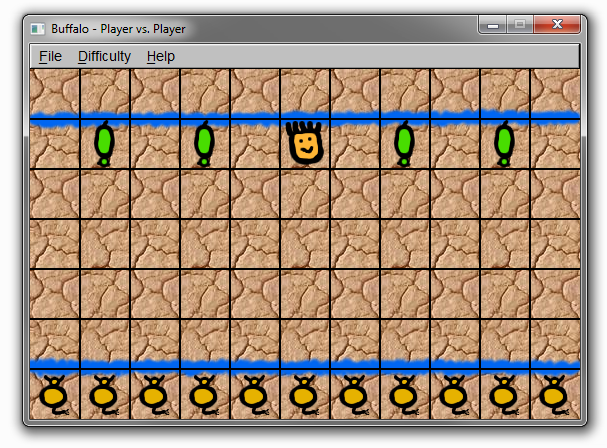
\includegraphics[height=0.4\textheight]{figure1.png}
	\end{center}
	\caption{A new player vs. player game from Buffalo. The buffalo must cross both rivers (indicated by the blue lines) to safety. If at least one buffalo crosses the second river, the buffalo win. Dogs and the indian may not cross either river.}
	\label{1}
\end{figure}
The game itself is based on an $11\times7$ \verb=grid= of \verb=char=s, which have no relation to the FLTK display except when prompted by an FLTK event. When a piece is moved, the \verb=grid= is consulted as to whether the move is valid. If another piece already inhabits the space the current piece is trying to use, the \verb=grid= returns the letter corresponding to that piece. If the \verb=grid= is unoccupied, it returns \verb=u=. Buffalo and dogs cannot move into a square that is occupied, however an indian can move into a space where a buffalo is held. The system used to update the \verb=grid= naturally deals with this as it essentially replaces the previous place of the piece with a \verb=u= and replaces the new co-ordinates with \verb=i= (or \verb=b= or \verb=d= for buffalo or dog respectively). Also, the FLTK interface forbids a dog or the indian to be placed beyond either river (see figure \ref{1}).

The FLTK interface itself is governed by switches inside the individual classes for the pieces. When a piece has an \verb=FL_PUSH= event above it, the piece is dragged along with the mouse until the button is released with an \verb=FL_RELEASE=. When released, the piece goes through several if loops: first to snap it to the \verb=grid=, and second to check if the move is valid. 

The game ends when either a buffalo crosses the second river, or all the buffalo are blocked by dogs and the Indian or are dead. When this happens, an \verb=Fl_choice= box pops up declaring the winner and gives the user a choice whether to start a new game versus human, new game versus computer or not to start a new game at all (causing the program to exit).

\begin{figure}[htb]
	\begin{center}
		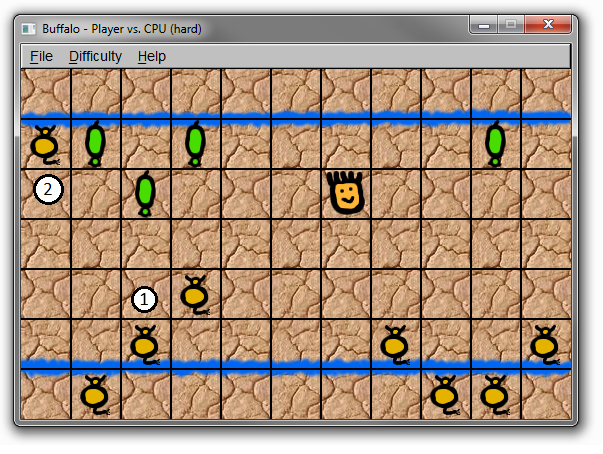
\includegraphics[height=0.4\textheight]{figure2.png}
	\end{center}
	\caption{A picture of Buffalo in progress. The three buffalo at 1 will not move as there is a dog in the same column as them. At 2, the buffalo will move forward next turn as he is unable to be stopped and the difficulty setting is on medium or greater.}
	\label{2}
\end{figure}
The AI is limited only to the buffalo and has three levels: random (easy); deterministic (medium); or a mixture of the two (hard). Random causes the buffalo to move randomly, but still respect the rules of the game. A buffalo will not approach a dog or indian i.e. the buffalo will not move if indian or dog is in the same column as itself (see figure \ref{2}). This is true for all levels of difficulty. Medium or deterministic difficulty calculates the buffalo furthest from the indian, and not blocked by another piece then moves it. The only exception to this is if the buffalo is one move away from winning, then it is instructed to take a winning move (see figure \ref{2}).  Hard level uses a mixture of these two methods by first determining which side of the board the indian is not in and second, choosing a random buffalo which can legally move from this half. The buffalo will still never approach a dog or Indian. Half is defined as half the range of movable buffalo.

There are several checks in place to make sure the user does not break the rules of the game. The first, already mentioned, is the inability for a piece to move outside of the rules of the game (i.e. over another piece or an illegal movement). The game also checks which player it is and if you try to move the peace that is not yours (or not the current player's) an \verb=Fl_message= pops up to protest and the piece is not moved. Third, dogs (the only piece to be able to move more than one square per turn) cannot move through other pieces. This is achieved by checking the \verb=grid= for pieces every square between the start position and the finish position.

The menubar is fairly standard. From the file menu, you can start a new game vs. human, new game versus CPU or quit. From the difficulty menu, you can select the difficulties previously discussed. The current mode of play can be seen in the title of the application. From the help menu you can access a PDF of the instructions and see the 'about' information.

\section{Limitations and Future Developments}
There are some base limitations of FLTK. One known bug is that if the mouse is pressed too quickly on an \verb=Fl_image=, the \verb=Fl_image= defaults to near (0,0).

Ideally, the game would incoporated a more intelligent AI (perhaps even learning), including an AI for the indian side.

The help would be encoporated into the FLTK program itself making the game more portable and searchable with tips on how to play etc..

A theme manager would also be a brilliant addition to the game, with dedicated theme files.

Sound would also add to the enjoyment of the game.
\section{Acknowledgements}
This game would not have been possible with FLTK if it were not for the patient effort of Ben Bradnick in teaching me its basic idioms. My thanks also goes to Mark Colclough and others in C++ lab (whose names I regrettably cannot recall) who have helped me understand the format of programming a GUI and have been, among other things, second eyes to check for mislaid pointers and arrays. 

\end{document}
